% Options for packages loaded elsewhere
% Options for packages loaded elsewhere
\PassOptionsToPackage{unicode}{hyperref}
\PassOptionsToPackage{hyphens}{url}
\PassOptionsToPackage{dvipsnames,svgnames,x11names}{xcolor}
%
\documentclass[
  letterpaper,
  DIV=11,
  numbers=noendperiod]{scrreprt}
\usepackage{xcolor}
\usepackage{amsmath,amssymb}
\setcounter{secnumdepth}{5}
\usepackage{iftex}
\ifPDFTeX
  \usepackage[T1]{fontenc}
  \usepackage[utf8]{inputenc}
  \usepackage{textcomp} % provide euro and other symbols
\else % if luatex or xetex
  \usepackage{unicode-math} % this also loads fontspec
  \defaultfontfeatures{Scale=MatchLowercase}
  \defaultfontfeatures[\rmfamily]{Ligatures=TeX,Scale=1}
\fi
\usepackage{lmodern}
\ifPDFTeX\else
  % xetex/luatex font selection
\fi
% Use upquote if available, for straight quotes in verbatim environments
\IfFileExists{upquote.sty}{\usepackage{upquote}}{}
\IfFileExists{microtype.sty}{% use microtype if available
  \usepackage[]{microtype}
  \UseMicrotypeSet[protrusion]{basicmath} % disable protrusion for tt fonts
}{}
\makeatletter
\@ifundefined{KOMAClassName}{% if non-KOMA class
  \IfFileExists{parskip.sty}{%
    \usepackage{parskip}
  }{% else
    \setlength{\parindent}{0pt}
    \setlength{\parskip}{6pt plus 2pt minus 1pt}}
}{% if KOMA class
  \KOMAoptions{parskip=half}}
\makeatother
% Make \paragraph and \subparagraph free-standing
\makeatletter
\ifx\paragraph\undefined\else
  \let\oldparagraph\paragraph
  \renewcommand{\paragraph}{
    \@ifstar
      \xxxParagraphStar
      \xxxParagraphNoStar
  }
  \newcommand{\xxxParagraphStar}[1]{\oldparagraph*{#1}\mbox{}}
  \newcommand{\xxxParagraphNoStar}[1]{\oldparagraph{#1}\mbox{}}
\fi
\ifx\subparagraph\undefined\else
  \let\oldsubparagraph\subparagraph
  \renewcommand{\subparagraph}{
    \@ifstar
      \xxxSubParagraphStar
      \xxxSubParagraphNoStar
  }
  \newcommand{\xxxSubParagraphStar}[1]{\oldsubparagraph*{#1}\mbox{}}
  \newcommand{\xxxSubParagraphNoStar}[1]{\oldsubparagraph{#1}\mbox{}}
\fi
\makeatother

\usepackage{color}
\usepackage{fancyvrb}
\newcommand{\VerbBar}{|}
\newcommand{\VERB}{\Verb[commandchars=\\\{\}]}
\DefineVerbatimEnvironment{Highlighting}{Verbatim}{commandchars=\\\{\}}
% Add ',fontsize=\small' for more characters per line
\usepackage{framed}
\definecolor{shadecolor}{RGB}{241,243,245}
\newenvironment{Shaded}{\begin{snugshade}}{\end{snugshade}}
\newcommand{\AlertTok}[1]{\textcolor[rgb]{0.68,0.00,0.00}{#1}}
\newcommand{\AnnotationTok}[1]{\textcolor[rgb]{0.37,0.37,0.37}{#1}}
\newcommand{\AttributeTok}[1]{\textcolor[rgb]{0.40,0.45,0.13}{#1}}
\newcommand{\BaseNTok}[1]{\textcolor[rgb]{0.68,0.00,0.00}{#1}}
\newcommand{\BuiltInTok}[1]{\textcolor[rgb]{0.00,0.23,0.31}{#1}}
\newcommand{\CharTok}[1]{\textcolor[rgb]{0.13,0.47,0.30}{#1}}
\newcommand{\CommentTok}[1]{\textcolor[rgb]{0.37,0.37,0.37}{#1}}
\newcommand{\CommentVarTok}[1]{\textcolor[rgb]{0.37,0.37,0.37}{\textit{#1}}}
\newcommand{\ConstantTok}[1]{\textcolor[rgb]{0.56,0.35,0.01}{#1}}
\newcommand{\ControlFlowTok}[1]{\textcolor[rgb]{0.00,0.23,0.31}{\textbf{#1}}}
\newcommand{\DataTypeTok}[1]{\textcolor[rgb]{0.68,0.00,0.00}{#1}}
\newcommand{\DecValTok}[1]{\textcolor[rgb]{0.68,0.00,0.00}{#1}}
\newcommand{\DocumentationTok}[1]{\textcolor[rgb]{0.37,0.37,0.37}{\textit{#1}}}
\newcommand{\ErrorTok}[1]{\textcolor[rgb]{0.68,0.00,0.00}{#1}}
\newcommand{\ExtensionTok}[1]{\textcolor[rgb]{0.00,0.23,0.31}{#1}}
\newcommand{\FloatTok}[1]{\textcolor[rgb]{0.68,0.00,0.00}{#1}}
\newcommand{\FunctionTok}[1]{\textcolor[rgb]{0.28,0.35,0.67}{#1}}
\newcommand{\ImportTok}[1]{\textcolor[rgb]{0.00,0.46,0.62}{#1}}
\newcommand{\InformationTok}[1]{\textcolor[rgb]{0.37,0.37,0.37}{#1}}
\newcommand{\KeywordTok}[1]{\textcolor[rgb]{0.00,0.23,0.31}{\textbf{#1}}}
\newcommand{\NormalTok}[1]{\textcolor[rgb]{0.00,0.23,0.31}{#1}}
\newcommand{\OperatorTok}[1]{\textcolor[rgb]{0.37,0.37,0.37}{#1}}
\newcommand{\OtherTok}[1]{\textcolor[rgb]{0.00,0.23,0.31}{#1}}
\newcommand{\PreprocessorTok}[1]{\textcolor[rgb]{0.68,0.00,0.00}{#1}}
\newcommand{\RegionMarkerTok}[1]{\textcolor[rgb]{0.00,0.23,0.31}{#1}}
\newcommand{\SpecialCharTok}[1]{\textcolor[rgb]{0.37,0.37,0.37}{#1}}
\newcommand{\SpecialStringTok}[1]{\textcolor[rgb]{0.13,0.47,0.30}{#1}}
\newcommand{\StringTok}[1]{\textcolor[rgb]{0.13,0.47,0.30}{#1}}
\newcommand{\VariableTok}[1]{\textcolor[rgb]{0.07,0.07,0.07}{#1}}
\newcommand{\VerbatimStringTok}[1]{\textcolor[rgb]{0.13,0.47,0.30}{#1}}
\newcommand{\WarningTok}[1]{\textcolor[rgb]{0.37,0.37,0.37}{\textit{#1}}}

\usepackage{longtable,booktabs,array}
\newcounter{none} % for unnumbered tables
\usepackage{calc} % for calculating minipage widths
% Correct order of tables after \paragraph or \subparagraph
\usepackage{etoolbox}
\makeatletter
\patchcmd\longtable{\par}{\if@noskipsec\mbox{}\fi\par}{}{}
\makeatother
% Allow footnotes in longtable head/foot
\IfFileExists{footnotehyper.sty}{\usepackage{footnotehyper}}{\usepackage{footnote}}
\makesavenoteenv{longtable}
\usepackage{graphicx}
\makeatletter
\newsavebox\pandoc@box
\newcommand*\pandocbounded[1]{% scales image to fit in text height/width
  \sbox\pandoc@box{#1}%
  \Gscale@div\@tempa{\textheight}{\dimexpr\ht\pandoc@box+\dp\pandoc@box\relax}%
  \Gscale@div\@tempb{\linewidth}{\wd\pandoc@box}%
  \ifdim\@tempb\p@<\@tempa\p@\let\@tempa\@tempb\fi% select the smaller of both
  \ifdim\@tempa\p@<\p@\scalebox{\@tempa}{\usebox\pandoc@box}%
  \else\usebox{\pandoc@box}%
  \fi%
}
% Set default figure placement to htbp
\def\fps@figure{htbp}
\makeatother





\setlength{\emergencystretch}{3em} % prevent overfull lines

\providecommand{\tightlist}{%
  \setlength{\itemsep}{0pt}\setlength{\parskip}{0pt}}



 


\KOMAoption{captions}{tableheading}
\makeatletter
\@ifpackageloaded{tcolorbox}{}{\usepackage[skins,breakable]{tcolorbox}}
\@ifpackageloaded{fontawesome5}{}{\usepackage{fontawesome5}}
\definecolor{quarto-callout-color}{HTML}{909090}
\definecolor{quarto-callout-note-color}{HTML}{0758E5}
\definecolor{quarto-callout-important-color}{HTML}{CC1914}
\definecolor{quarto-callout-warning-color}{HTML}{EB9113}
\definecolor{quarto-callout-tip-color}{HTML}{00A047}
\definecolor{quarto-callout-caution-color}{HTML}{FC5300}
\definecolor{quarto-callout-color-frame}{HTML}{acacac}
\definecolor{quarto-callout-note-color-frame}{HTML}{4582ec}
\definecolor{quarto-callout-important-color-frame}{HTML}{d9534f}
\definecolor{quarto-callout-warning-color-frame}{HTML}{f0ad4e}
\definecolor{quarto-callout-tip-color-frame}{HTML}{02b875}
\definecolor{quarto-callout-caution-color-frame}{HTML}{fd7e14}
\makeatother
\makeatletter
\@ifpackageloaded{bookmark}{}{\usepackage{bookmark}}
\makeatother
\makeatletter
\@ifpackageloaded{caption}{}{\usepackage{caption}}
\AtBeginDocument{%
\ifdefined\contentsname
  \renewcommand*\contentsname{Table of contents}
\else
  \newcommand\contentsname{Table of contents}
\fi
\ifdefined\listfigurename
  \renewcommand*\listfigurename{List of Figures}
\else
  \newcommand\listfigurename{List of Figures}
\fi
\ifdefined\listtablename
  \renewcommand*\listtablename{List of Tables}
\else
  \newcommand\listtablename{List of Tables}
\fi
\ifdefined\figurename
  \renewcommand*\figurename{Figure}
\else
  \newcommand\figurename{Figure}
\fi
\ifdefined\tablename
  \renewcommand*\tablename{Table}
\else
  \newcommand\tablename{Table}
\fi
}
\@ifpackageloaded{float}{}{\usepackage{float}}
\floatstyle{ruled}
\@ifundefined{c@chapter}{\newfloat{codelisting}{h}{lop}}{\newfloat{codelisting}{h}{lop}[chapter]}
\floatname{codelisting}{Listing}
\newcommand*\listoflistings{\listof{codelisting}{List of Listings}}
\makeatother
\makeatletter
\makeatother
\makeatletter
\@ifpackageloaded{caption}{}{\usepackage{caption}}
\@ifpackageloaded{subcaption}{}{\usepackage{subcaption}}
\makeatother
\usepackage{bookmark}
\IfFileExists{xurl.sty}{\usepackage{xurl}}{} % add URL line breaks if available
\urlstyle{same}
\hypersetup{
  pdftitle={Spikes in your face},
  pdfauthor={Joseph Ziminski; Please add your name here},
  colorlinks=true,
  linkcolor={blue},
  filecolor={Maroon},
  citecolor={Blue},
  urlcolor={Blue},
  pdfcreator={LaTeX via pandoc}}


\title{Spikes in your face}
\author{Joseph Ziminski \and Please add your name here}
\date{2027-03-04}
\begin{document}
\maketitle

\renewcommand*\contentsname{Table of contents}
{
\setcounter{tocdepth}{2}
\tableofcontents
}

\bookmarksetup{startatroot}

\chapter*{Preface}\label{preface}
\addcontentsline{toc}{chapter}{Preface}

\markboth{Preface}{Preface}

Welcome to spikes in your face! This course will tell you all about
spikes.

This page should include: 1) Introduction to the course and its purpose
2) Schedule for the course (can be removed after the course) 3)
Versioning 4) Funding

Spikes \& Signals Spike Sorting in Practice Spikes \& Signals: A
Practical Course in Spike Sorting Spikes \& Signals: Spike Sorting
Pipelines with SpikeInterface From Noise to Neurons Order from Chaos:
\ldots{} Finding Neurons in the Noise

To learn more about Quarto books visit
\url{https://quarto.org/docs/books}.

\bookmarksetup{startatroot}

\chapter*{Introduction}\label{introduction}
\addcontentsline{toc}{chapter}{Introduction}

\markboth{Introduction}{Introduction}

\section*{Why do we do extracellular
electrophysiology?}\label{why-do-we-do-extracellular-electrophysiology}
\addcontentsline{toc}{section}{Why do we do extracellular
electrophysiology?}

\markright{Why do we do extracellular electrophysiology?}

\section*{Neurons, spikes and the extracellular
signal}\label{neurons-spikes-and-the-extracellular-signal}
\addcontentsline{toc}{section}{Neurons, spikes and the extracellular
signal}

\markright{Neurons, spikes and the extracellular signal}

\section*{Recording from the extracellular
space}\label{recording-from-the-extracellular-space}
\addcontentsline{toc}{section}{Recording from the extracellular space}

\markright{Recording from the extracellular space}

\subsection*{The recording set up}\label{the-recording-set-up}
\addcontentsline{toc}{subsection}{The recording set up}

\subsection*{High-density probes}\label{high-density-probes}
\addcontentsline{toc}{subsection}{High-density probes}

\section*{The acquired data}\label{the-acquired-data}
\addcontentsline{toc}{section}{The acquired data}

\markright{The acquired data}

\section*{An overview of the spike-sorting
pipeline}\label{an-overview-of-the-spike-sorting-pipeline}
\addcontentsline{toc}{section}{An overview of the spike-sorting
pipeline}

\markright{An overview of the spike-sorting pipeline}

(can introduce SpikeInterface here)

\section*{Linking spikes to
behaviour}\label{linking-spikes-to-behaviour}
\addcontentsline{toc}{section}{Linking spikes to behaviour}

\markright{Linking spikes to behaviour}

GEneral Notes \textsuperscript{}CHECK THIS (LOWER)
https://pmc.ncbi.nlm.nih.gov/articles/PMC3715549/\#:\textasciitilde:text=Note\%20that\%20we\%20here\%20for,setup\%20and\%20the\%20mathematical\%20model.
https://d.lib.msu.edu/etd/10273?\_\_goaway\_challenge=header-refresh\&\_\_goaway\_id=ca01fdb6671dc71b62462ce092b4bbd1\&\_\_goaway\_referer=https\%3A\%2F\%2Fd.lib.msu.edu\%2F
(HIGHH 1k-5k)

\bookmarksetup{startatroot}

\chapter*{Walking through a SpikeInterface
pipeline}\label{walking-through-a-spikeinterface-pipeline}
\addcontentsline{toc}{chapter}{Walking through a SpikeInterface
pipeline}

\markboth{Walking through a SpikeInterface pipeline}{Walking through a
SpikeInterface pipeline}

\hfill\break
In this chapter, we will code an entire spike sorting pipeline using
SpikeInterface. We will load and preprocesing the data, run spike
sorting and compute metrics for assessing the sorting quality.

In this walkthrough, we will use an example dataset available
\href{}{here}. This dataset contains XXX minutes of data recorded on 384
channels, located on the middle two shanks of a 4-shank Neuropixels
probe, acquired in SpikeGLX.

ADD THE COMPELTELED WALKTHROUGH. SAY DON'T COPY. DONT USE AI. TYPE IT
ALL.

\section*{Section 1: Loading and data
exploration}\label{section-1-loading-and-data-exploration}
\addcontentsline{toc}{section}{Section 1: Loading and data exploration}

\markright{Section 1: Loading and data exploration}

\section*{Loading the data}\label{loading-the-data}
\addcontentsline{toc}{section}{Loading the data}

\markright{Loading the data}

SpikeInterface can load data from many different types of acquisition
systems, using functions within its
\href{https://spikeinterface.readthedocs.io/en/stable/modules/extractors.html}{extractors
module}. As our data is from SpikeGLX, we will use the
\texttt{read\_spikeglx} method.

We need to tell SpikeInterfafce where the data is, and what
\href{https://github.com/billkarsh/SpikeGLX/blob/master/Markdown/UserManual.md\#data-stream}{data
stream} we want to load.

Streams written by SpikeGLX can include the action potential (AP) band,
local feild potential (LF) band and a sync stream. Because we want to
load the AP data stream for spike sorting, we pass \texttt{"imec0.ap"}.

\begin{tcolorbox}[enhanced jigsaw, arc=.35mm, bottomrule=.15mm, bottomtitle=1mm, breakable, colback=white, colbacktitle=quarto-callout-note-color!10!white, colframe=quarto-callout-note-color-frame, coltitle=black, left=2mm, leftrule=.75mm, opacityback=0, opacitybacktitle=0.6, rightrule=.15mm, title=\textcolor{quarto-callout-note-color}{\faInfo}\hspace{0.5em}{Details on SpikeGLX streams}, titlerule=0mm, toprule=.15mm, toptitle=1mm]

In earlier versions of Neuropixels probes, the data was filtered in the
probe into two separate streams. The action potential (AP) band was
filtered with high-pass filter (300, 500 or 1000 Hz depending on
settings). This removes low-frequency component, keeping the action
potentials (which are typically in the 300-3000Hz range) untouched. This
stream was used for spike sorting.

https://github.com/billkarsh/SpikeGLX/blob/master/Markdown/UserManual.md\#data-stream

\textsuperscript{}CHECK THIS (LOWER)
https://pmc.ncbi.nlm.nih.gov/articles/PMC3715549/\#:\textasciitilde:text=Note\%20that\%20we\%20here\%20for,setup\%20and\%20the\%20mathematical\%20model.
https://d.lib.msu.edu/etd/10273?\_\_goaway\_challenge=header-refresh\&\_\_goaway\_id=ca01fdb6671dc71b62462ce092b4bbd1\&\_\_goaway\_referer=https\%3A\%2F\%2Fd.lib.msu.edu\%2F
(HIGHH 1k-5k)

A local-field potential band was also written, filtered using a 300 Hz
low pass filter. This removes high-frequency data (including action
potential) and left low-freuqnecy local feild potential (LF). The LF
band represents the summed oscilatiosn of votlage from across the brain
and is subject to differnt analysiss.

In more recent Neuropixels versions (e.g.~Neuropixels 2) there is no
logner a distinction betweeen data streams. The unfiltered data is
written to disk (saved in the \texttt{imec0.ap} band suffix, although it
is now broadband), and popst-hoc filtering left up to the user.

There is also a sync stream. that records a digital sync signal. This
allows you to align the neural data to external events (behaviour,
stimuli, other data streams, or other probes) by embedding shared TTL
pulses into the recording.

\end{tcolorbox}

\begin{Shaded}
\begin{Highlighting}[]
\ImportTok{import}\NormalTok{ spikeinterface.extractors }\ImportTok{as}\NormalTok{ si\_extractors}

\CommentTok{\# This should be the path to the folder contaning}
\CommentTok{\# the data. On Windows, you may need to preprend}
\CommentTok{\# r to the string e.g. r"C:\textbackslash{}my\textbackslash{}path"}
\NormalTok{path\_to\_data\_folder }\OperatorTok{=} \StringTok{"data/pipeline{-}walkthrough"}

\NormalTok{recording }\OperatorTok{=}\NormalTok{ si\_extractors.read\_spikeglx(}
\NormalTok{    path\_to\_data\_folder,}
\NormalTok{    stream\_id}\OperatorTok{=}\StringTok{"imec0.ap"}
\NormalTok{)}

\BuiltInTok{print}\NormalTok{(recording)}
\end{Highlighting}
\end{Shaded}

\begin{verbatim}
SpikeGLXRecordingExtractor: 384 channels - 30.0kHz - 1 segments - 75,000 samples - 2.50s 
                            int16 dtype - 54.93 MiB
\end{verbatim}

The loading functions return the \texttt{recording} as a Python object,
which contains many useful methods for exploring the recording metadata
as well as accessing the underlying data.

\begin{tcolorbox}[enhanced jigsaw, arc=.35mm, bottomrule=.15mm, bottomtitle=1mm, breakable, colback=white, colbacktitle=quarto-callout-note-color!10!white, colframe=quarto-callout-note-color-frame, coltitle=black, left=2mm, leftrule=.75mm, opacityback=0, opacitybacktitle=0.6, rightrule=.15mm, title=\textcolor{quarto-callout-note-color}{\faInfo}\hspace{0.5em}{Details on class inheritence in SpikeInterface}, titlerule=0mm, toprule=.15mm, toptitle=1mm]

Under the hood, SpikeInterface XX widely relies on a class inheritence
model, and the \texttt{Recording} object is a good example of this. A
\texttt{BaseRecording} object defines many useful functions for
interacting with a recording for example \texttt{getXXX} (see the API
docs here). All other recording objects inherit from this BaseRcording
object, for example our SpiekGLXRecordingExtractor object inherits from
BaseRecording, and so contains all of this.

Every recording-like object we will deal with doday inherits from
BaseRecording and so includes all this functionality. Often, these
inherited classes add some functinoaity on top. For example,
\texttt{BaseRecording} has a \texttt{get\_traces()} fucntion that
returns the underlying data. A Filter recording extends this function to
first filter the data before returning it.

\end{tcolorbox}

\subsection*{Exploring the Recording
object}\label{exploring-the-recording-object}
\addcontentsline{toc}{subsection}{Exploring the Recording object}

The recording object is a
\href{https://www.reddit.com/r/learnprogramming/comments/uekqvv/comment/i6ns974/?utm_source=share&utm_medium=web3x&utm_name=web3xcss&utm_term=1&utm_content=share_button}{Python
object} contaning maybe useful methods. The
\href{https://spikeinterface.readthedocs.io/en/latest/api.html}{SpikeInterface
API Documentation} is a useful resource for looking up methods
associated with an object and their arguments. TODO MENTION
BASERECORDING.

You can also use Python's \texttt{dir()} functoin to see all attributes
and methods associated with any Python object.

\begin{Shaded}
\begin{Highlighting}[]
\BuiltInTok{print}\NormalTok{(}
\NormalTok{    [method }\ControlFlowTok{for}\NormalTok{ method }\KeywordTok{in} \BuiltInTok{dir}\NormalTok{(recording) }\ControlFlowTok{if}\NormalTok{ method.startswith(}\StringTok{"get"}\NormalTok{)]}
\NormalTok{)}
\end{Highlighting}
\end{Shaded}

\begin{verbatim}
['get_annotation', 'get_annotation_keys', 'get_binary_description', 'get_channel_gains', 'get_channel_groups', 'get_channel_ids', 'get_channel_locations', 'get_channel_offsets', 'get_channel_property', 'get_dtype', 'get_duration', 'get_end_time', 'get_memory_size', 'get_neo_io_reader', 'get_num_blocks', 'get_num_channels', 'get_num_frames', 'get_num_samples', 'get_num_segments', 'get_parent', 'get_preferred_mp_context', 'get_probe', 'get_probegroup', 'get_probes', 'get_property', 'get_property_keys', 'get_sampling_frequency', 'get_start_time', 'get_streams', 'get_time_info', 'get_times', 'get_total_duration', 'get_total_memory_size', 'get_total_samples', 'get_traces']
\end{verbatim}

\begin{tcolorbox}[enhanced jigsaw, arc=.35mm, bottomrule=.15mm, bottomtitle=1mm, breakable, colback=white, colbacktitle=quarto-callout-tip-color!10!white, colframe=quarto-callout-tip-color-frame, coltitle=black, left=2mm, leftrule=.75mm, opacityback=0, opacitybacktitle=0.6, rightrule=.15mm, title=\textcolor{quarto-callout-tip-color}{\faLightbulb}\hspace{0.5em}{Some things to try}, titlerule=0mm, toprule=.15mm, toptitle=1mm]

This is a good time to play around with the \texttt{recording}, using
the API docs
(\href{https://spikeinterface.readthedocs.io/en/latest/api.html\#spikeinterface.core.BaseRecording}{BaseRecording
object}) to navigate it. Have a go at:

\begin{enumerate}
\def\labelenumi{\arabic{enumi}.}
\tightlist
\item
  Print the locations of all channels on the probe.
\item
  Print the time vector associated with the recording.
\item
  Use \texttt{get\_traces()} to retrieve a segment of the raw data as a
  NumPy array. What are its dimensions?
\end{enumerate}

\end{tcolorbox}

\subsection*{Visualising the probe}\label{visualising-the-probe}
\addcontentsline{toc}{subsection}{Visualising the probe}

There are many different types of probe used in extracellular
electrophysiology (e.g.~
\href{https://www.neuropixels.org/}{Neuropixels},
\href{https://www.cambridgeneurotech.com/neural-probes}{Cambridge
Neurotech},
\href{https://www.neuronexus.com/products/electrode-arrays/}{NeuroNexus}
). They can come in very complex arrangements. Probeinterface is a
library used by SpikeInterface (and by the same developers) to load many
different types of probe.

It is important to check that your probe has loaded as expected, and
that the geometry matches how it was set up in your acquisition
software. To do this, we can plot the probe to confirm it loaded
correctly:

\begin{Shaded}
\begin{Highlighting}[]
\ImportTok{from}\NormalTok{ probeinterface.plotting }\ImportTok{import}\NormalTok{ plot\_probe}
\ImportTok{import}\NormalTok{ matplotlib.pyplot }\ImportTok{as}\NormalTok{ plt}

\NormalTok{probe }\OperatorTok{=}\NormalTok{ recording.get\_probe()}

\NormalTok{plot\_probe(probe)}
\NormalTok{plt.show()}
\end{Highlighting}
\end{Shaded}

\pandocbounded{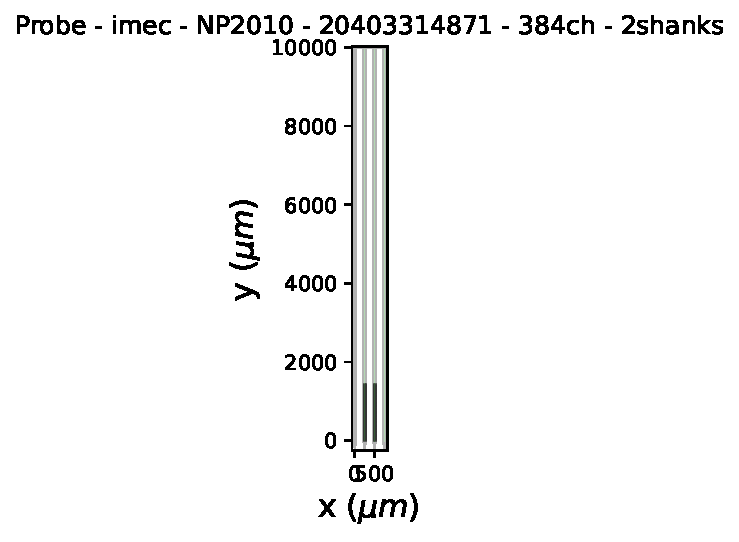
\includegraphics[keepaspectratio]{pipeline-walkthrough_files/figure-pdf/cell-4-output-1.pdf}}

Here we can see we have a two-shank Neuropixels probe with recording
sites on the two central shanks, as was expected. You can also use the
\texttt{show\_contact\_ids} argument to display the contact IDs, to
double check the exact location of each contact.

\subsection*{Visualising the data}\label{visualising-the-data}
\addcontentsline{toc}{subsection}{Visualising the data}

Extracellula relectrophysiological data is suceptible to many noise
sources, including electrical noise, phyical noise from movements in the
probe as well as phyiscal issues with the probe (?).

As such, it is important to visualise the data, especially after
preprocessing, to check the data quality. First, lets's plot one second
of data from our raw recording:

\begin{Shaded}
\begin{Highlighting}[]
\ImportTok{import}\NormalTok{ spikeinterface.widgets }\ImportTok{as}\NormalTok{ si\_widgets}

\NormalTok{start\_time }\OperatorTok{=}\NormalTok{ recording.get\_times()[}\DecValTok{0}\NormalTok{]}

\NormalTok{si\_widgets.plot\_traces(}
\NormalTok{    recording,}
\NormalTok{    time\_range}\OperatorTok{=}\NormalTok{(start\_time, start\_time }\OperatorTok{+} \FloatTok{0.1}\NormalTok{),}
\NormalTok{    return\_in\_uV}\OperatorTok{=}\VariableTok{True}\NormalTok{,}
\NormalTok{    order\_channel\_by\_depth}\OperatorTok{=}\VariableTok{True}
\NormalTok{)}
\NormalTok{plt.show()}
\end{Highlighting}
\end{Shaded}

\pandocbounded{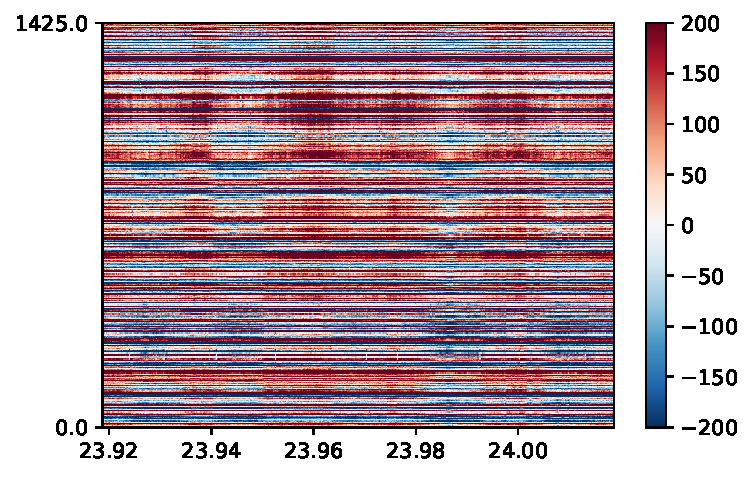
\includegraphics[keepaspectratio]{pipeline-walkthrough_files/figure-pdf/cell-5-output-1.pdf}}

Here we return in \texttt{uV} to ensure the data is returned in
interpretable units, and use \texttt{order\_channel\_by\_depth} as the
default ordering of channels on the probe is not always by depth (WHY?
represents how stored by acquisition system?)

As we can see - the data looks terrible! It is contaiminated with sever
electrical noise and other issues. We will need to preprocess it to tidy
it up.

\begin{tcolorbox}[enhanced jigsaw, arc=.35mm, bottomrule=.15mm, bottomtitle=1mm, breakable, colback=white, colbacktitle=quarto-callout-note-color!10!white, colframe=quarto-callout-note-color-frame, coltitle=black, left=2mm, leftrule=.75mm, opacityback=0, opacitybacktitle=0.6, rightrule=.15mm, title=\textcolor{quarto-callout-note-color}{\faInfo}\hspace{0.5em}{A note on scaling to \texttt{uV}}, titlerule=0mm, toprule=.15mm, toptitle=1mm]

Most acquisition systems will store data in \texttt{int16} format
(i.e.~integers in the range XXX) to save storage space. To get these
values, the acquired data in \texttt{uV} is scaled and offset into the
\texttt{int16} range.

By default, SpikeInterface will display the raw \texttt{int16} data. To
use the stored offsets and gains to reconstrct XX, we can use the
\texttt{return\_in\_uV} argument on many functions. Also see XX, XX and
XX for working with these.

\end{tcolorbox}

\section*{Section 2: Preprocessing}\label{section-2-preprocessing}
\addcontentsline{toc}{section}{Section 2: Preprocessing}

\markright{Section 2: Preprocessing}

To preprocess the data, we will pass our recording object into functions
that return a new, recording object.
e.g.~\texttt{filtered\_recording\ =\ bandpass\_filter(recording)}.

This is almost instantenous as all preprocessing is applied `lazily'.
When we apply the preprocessing function, we just change the metadata
associated with the recording. Only when we get the data (e.g.~in
\texttt{plot\_traces}, or with \texttt{get\_traces()} or when saving the
data) is the data preprocessed in the requested chunk. This makes
operating very fast!

Below, we will apply three key preprocessing steps. In the next chapter,
we will dive into more detail on the theory of these steps and inrtoduce
more.

\textbf{phase\_shift} : corrects a hardware artefact in the Neuropixels
probe which causes small shifts between the recording time across nearby
channels.

\textbf{bandpass\_filter} : removes high and low frequency oscillations
from the data. It is applied to each channel separately.

\textbf{commmon\_reference} : removes noise spikes that appear as
verticle stripes across the data. It is applied across channels
separately at each timepoint.

We can easily apply these preprocessing steps with the processing
module:

\begin{Shaded}
\begin{Highlighting}[]
\ImportTok{import}\NormalTok{ spikeinterface.preprocessing }\ImportTok{as}\NormalTok{ si\_prepro}

\NormalTok{phase\_shift\_recording }\OperatorTok{=}\NormalTok{ si\_prepro.phase\_shift(recording)}
\NormalTok{filtered\_recording }\OperatorTok{=}\NormalTok{ si\_prepro.bandpass\_filter(}
\NormalTok{    phase\_shift\_recording, freq\_min}\OperatorTok{=}\DecValTok{300}\NormalTok{, freq\_max}\OperatorTok{=}\DecValTok{6000}
\NormalTok{)}
\NormalTok{cmr\_recording }\OperatorTok{=}\NormalTok{ si\_prepro.common\_reference(}
\NormalTok{    filtered\_recording, operator}\OperatorTok{=}\StringTok{"median"}
\NormalTok{)}
\end{Highlighting}
\end{Shaded}

Cool, we can plot the data:

\begin{Shaded}
\begin{Highlighting}[]
\NormalTok{si\_widgets.plot\_traces(}
\NormalTok{    cmr\_recording,}
\NormalTok{    time\_range}\OperatorTok{=}\NormalTok{(start\_time, start\_time }\OperatorTok{+} \FloatTok{0.1}\NormalTok{),}
\NormalTok{    return\_in\_uV}\OperatorTok{=}\VariableTok{True}\NormalTok{,}
\NormalTok{    order\_channel\_by\_depth}\OperatorTok{=}\VariableTok{True}
\NormalTok{)}
\NormalTok{plt.show()}
\end{Highlighting}
\end{Shaded}

\pandocbounded{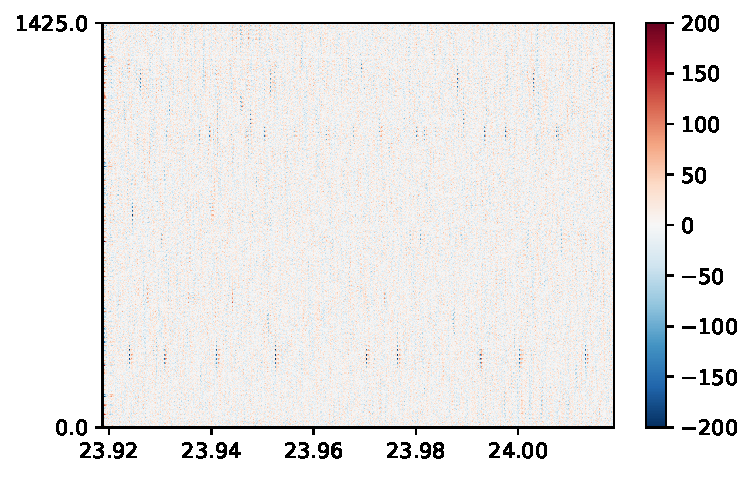
\includegraphics[keepaspectratio]{pipeline-walkthrough_files/figure-pdf/cell-7-output-1.pdf}}

\begin{tcolorbox}[enhanced jigsaw, arc=.35mm, bottomrule=.15mm, bottomtitle=1mm, breakable, colback=white, colbacktitle=quarto-callout-tip-color!10!white, colframe=quarto-callout-tip-color-frame, coltitle=black, left=2mm, leftrule=.75mm, opacityback=0, opacitybacktitle=0.6, rightrule=.15mm, title=\textcolor{quarto-callout-tip-color}{\faLightbulb}\hspace{0.5em}{Something to try}, titlerule=0mm, toprule=.15mm, toptitle=1mm]

Can you: - try plotting the data after each preprocessing step, to see
the effect of each - ANYTHING ELSE?

\end{tcolorbox}

\subsection*{Splitting the data by
shank}\label{splitting-the-data-by-shank}
\addcontentsline{toc}{subsection}{Splitting the data by shank}

You might notice the data in the above image looks slightly strange. All
spikes have predictable gaps between them:

\begin{Shaded}
\begin{Highlighting}[]
\NormalTok{si\_widgets.plot\_traces(}
\NormalTok{    cmr\_recording,}
\NormalTok{    time\_range}\OperatorTok{=}\NormalTok{(}\FloatTok{23.923}\NormalTok{, }\FloatTok{23.928}\NormalTok{),}
\NormalTok{    return\_in\_uV}\OperatorTok{=}\VariableTok{True}\NormalTok{,}
\NormalTok{    order\_channel\_by\_depth}\OperatorTok{=}\VariableTok{True}\NormalTok{,}
\NormalTok{)}
\NormalTok{ax }\OperatorTok{=}\NormalTok{ plt.gca()}
\NormalTok{ax.set\_ylim(}\DecValTok{200}\NormalTok{, }\DecValTok{300}\NormalTok{)}
\NormalTok{plt.show()}
\end{Highlighting}
\end{Shaded}

\pandocbounded{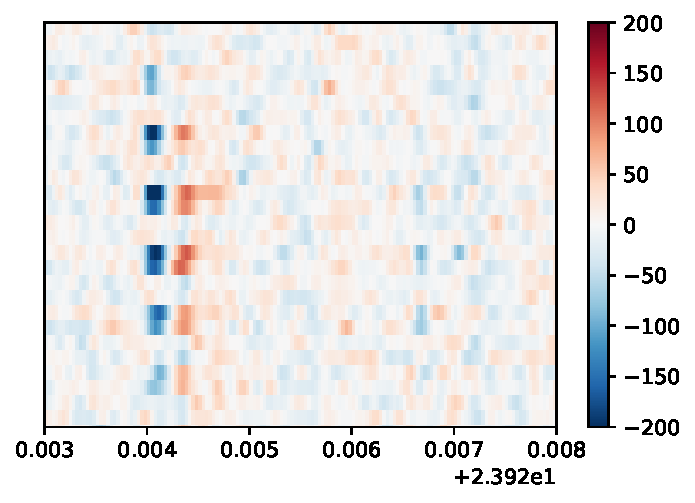
\includegraphics[keepaspectratio]{pipeline-walkthrough_files/figure-pdf/cell-8-output-1.pdf}}

\begin{tcolorbox}[enhanced jigsaw, arc=.35mm, bottomrule=.15mm, bottomtitle=1mm, breakable, colback=white, colbacktitle=quarto-callout-note-color!10!white, colframe=quarto-callout-note-color-frame, coltitle=black, left=2mm, leftrule=.75mm, opacityback=0, opacitybacktitle=0.6, rightrule=.15mm, title={Why does the data look like this?}, titlerule=0mm, toprule=.15mm, toptitle=1mm]

Look carefully at the plot above. Why do you think there are predictable
gaps in the signal every two channels?

\end{tcolorbox}

\begin{tcolorbox}[enhanced jigsaw, arc=.35mm, bottomrule=.15mm, bottomtitle=1mm, breakable, colback=white, colbacktitle=quarto-callout-note-color!10!white, colframe=quarto-callout-note-color-frame, coltitle=black, left=2mm, leftrule=.75mm, opacityback=0, opacitybacktitle=0.6, rightrule=.15mm, title=\textcolor{quarto-callout-note-color}{\faInfo}\hspace{0.5em}{Click to reveal the answer}, titlerule=0mm, toprule=.15mm, toptitle=1mm]

For many probes, it is normal to have slight differences between
adjacent channels because they are often in column format. One column
can get a stronger signal than another.

Here however there is significantly different signal every two channels.
This is because we are plotting all shanks together, in y-axis order. So
different shanks are interspersed.

\end{tcolorbox}

We can solve this by spliting the recording by shank with the
\texttt{groups} property. When SpikeInterface loads the data, it will
automatically assign different shanks to different groups.

\begin{Shaded}
\begin{Highlighting}[]
\NormalTok{split\_recording }\OperatorTok{=}\NormalTok{ cmr\_recording.split\_by(}\StringTok{"group"}\NormalTok{)}
\BuiltInTok{print}\NormalTok{(}
\NormalTok{    split\_recording}
\NormalTok{)}
\end{Highlighting}
\end{Shaded}

\begin{verbatim}
{0: ChannelSliceRecording: 192 channels - 30.0kHz - 1 segments - 75,000 samples - 2.50s - int16 dtype 
                       27.47 MiB, 1: ChannelSliceRecording: 192 channels - 30.0kHz - 1 segments - 75,000 samples - 2.50s - int16 dtype 
                       27.47 MiB}
\end{verbatim}

We can plot both shanks separately:

\begin{Shaded}
\begin{Highlighting}[]
\NormalTok{fig, ax }\OperatorTok{=}\NormalTok{ plt.subplots(}\DecValTok{1}\NormalTok{, }\DecValTok{2}\NormalTok{)}

\ControlFlowTok{for}\NormalTok{ shank\_idx, shank\_recording }\KeywordTok{in}\NormalTok{ split\_recording.items():}

\NormalTok{    si\_widgets.plot\_traces(}
\NormalTok{        shank\_recording,}
\NormalTok{        time\_range}\OperatorTok{=}\NormalTok{(start\_time, start\_time }\OperatorTok{+} \FloatTok{0.1}\NormalTok{),}
\NormalTok{        return\_in\_uV}\OperatorTok{=}\VariableTok{True}\NormalTok{,}
\NormalTok{        order\_channel\_by\_depth}\OperatorTok{=}\VariableTok{True}\NormalTok{,}
\NormalTok{        ax}\OperatorTok{=}\NormalTok{ax[shank\_idx]}
\NormalTok{    )}
\NormalTok{    ax[shank\_idx].set\_title(}\SpecialStringTok{f"Shank: }\SpecialCharTok{\{}\NormalTok{shank\_idx}\SpecialCharTok{\}}\SpecialStringTok{"}\NormalTok{)}

\NormalTok{plt.show()}
\end{Highlighting}
\end{Shaded}

\pandocbounded{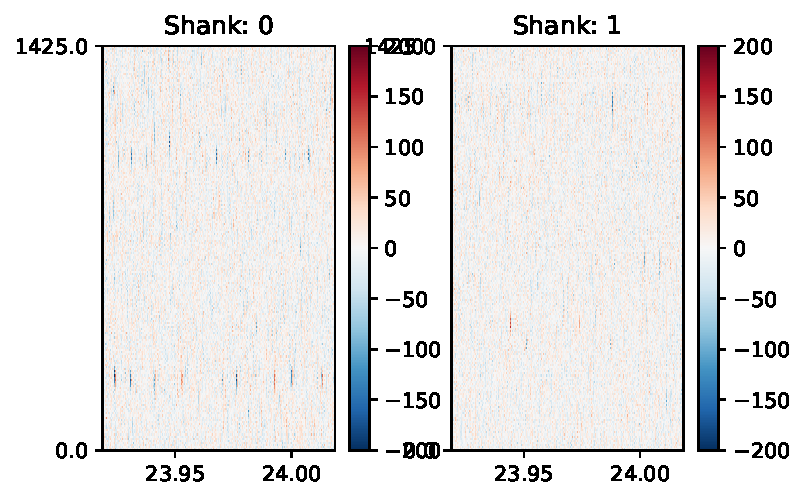
\includegraphics[keepaspectratio]{pipeline-walkthrough_files/figure-pdf/cell-10-output-1.pdf}}

Much better!

Now we have our preprocessed data, and have visually confirmed the data
quality is good, we are ready to perform spike sorting!

\subsection*{Additional things to try}\label{additional-things-to-try}
\addcontentsline{toc}{subsection}{Additional things to try}

Here are some optional tasks to try to furthe familiarlise yourself with
preprocessing in spikeinterface.

\section*{Section 2: Sorting}\label{section-2-sorting}
\addcontentsline{toc}{section}{Section 2: Sorting}

\markright{Section 2: Sorting}

What we are fundamentally interested in doing is XXX.

Now we are ready to move onto spike sorting. In our data, we can see by
eye the action potentials recorded on the probe:

\pandocbounded{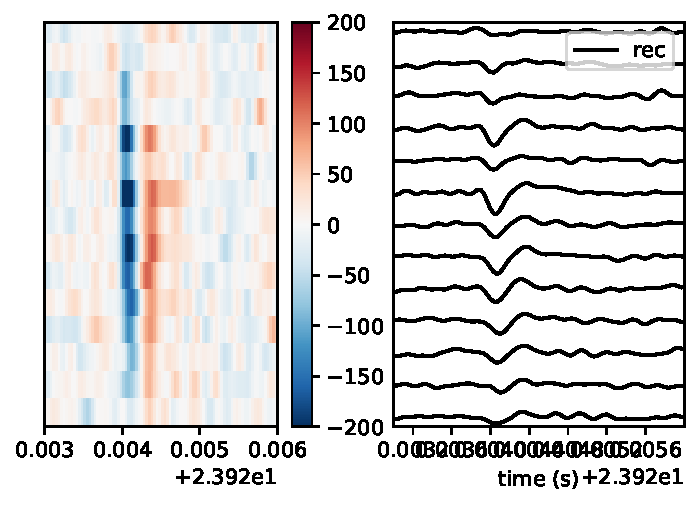
\includegraphics[keepaspectratio]{pipeline-walkthrough_files/figure-pdf/cell-11-output-1.pdf}}

A close up of a single action potential on the probe.

Although we can easily indetify these by eye, it is the sorters job both
to algorithmically detect these action potentials (hereforth called
`spikes') and separate them. XXX

In this schematic, \ldots.

In SpikeInterface, running a sorter is quite simple. Today, we will run
Kilosort4, and we can do it with a single function call:

\begin{Shaded}
\begin{Highlighting}[]
\ImportTok{import}\NormalTok{ spikeinterface.sorters }\ImportTok{as}\NormalTok{ si\_sorters}

\NormalTok{sorting }\OperatorTok{=}\NormalTok{ si\_sorters.run\_sorter(}
    \StringTok{"kilosort4"}\NormalTok{,}
\NormalTok{    cmr\_recording,}
\NormalTok{    remove\_existing\_folder}\OperatorTok{=}\VariableTok{True}\NormalTok{,}
\NormalTok{    do\_CAR}\OperatorTok{=}\VariableTok{False}\NormalTok{,}
\NormalTok{    highpass\_cutoff}\OperatorTok{=}\FloatTok{0.1}\NormalTok{,}
\NormalTok{)}

\BuiltInTok{print}\NormalTok{(sorting)}
\end{Highlighting}
\end{Shaded}

\begin{verbatim}

  0%|          | 0/2 [00:00<?, ?it/s]
 50%|█████     | 1/2 [00:05<00:05,  5.84s/it]
100%|██████████| 2/2 [00:11<00:00,  5.46s/it]
100%|██████████| 2/2 [00:11<00:00,  5.52s/it]

  0%|          | 0/2 [00:00<?, ?it/s]
 50%|█████     | 1/2 [00:05<00:05,  5.82s/it]
100%|██████████| 2/2 [00:11<00:00,  5.62s/it]
100%|██████████| 2/2 [00:11<00:00,  5.65s/it]

  0%|          | 0/2 [00:00<?, ?it/s]
 50%|█████     | 1/2 [00:00<00:00, 32.19it/s]
100%|██████████| 2/2 [00:00<00:00, 31.84it/s]
100%|██████████| 2/2 [00:00<00:00, 31.55it/s]

  0%|          | 0/2 [00:00<?, ?it/s]
 50%|█████     | 1/2 [00:01<00:01,  1.52s/it]
100%|██████████| 2/2 [00:02<00:00,  1.33s/it]
100%|██████████| 2/2 [00:02<00:00,  1.36s/it]

  0%|          | 0/2 [00:00<?, ?it/s]
 50%|█████     | 1/2 [00:00<00:00, 42.86it/s]
100%|██████████| 2/2 [00:00<00:00, 50.80it/s]
100%|██████████| 2/2 [00:00<00:00, 48.63it/s]
\end{verbatim}

\begin{verbatim}
KiloSortSortingExtractor: 83 units - 1 segments - 30.0kHz
\end{verbatim}

You will see the sorting output written to disk. This contains all of
the output files of the sorter. We will go through these outputs in
detail XXX. The key outputs are \texttt{spike\_times.npy}, and
\texttt{spike\_clusters.npy}. EXPLAIN

We also have this information in a spikeinterface \texttt{sorting}
object. We can get it e.g.:

SPIKE TIMES SPIKE CLUSTERS

\section*{Section 4: Postprocessing}\label{section-4-postprocessing}
\addcontentsline{toc}{section}{Section 4: Postprocessing}

\markright{Section 4: Postprocessing}

This will be a whitestop tour. We will go into much more detail later.
What is teh purpose of this.

\subsection*{create sorting analyzer}\label{create-sorting-analyzer}
\addcontentsline{toc}{subsection}{create sorting analyzer}

In SPikeInterface, the main construct for work with postprocessing of
spike sorting outputs is the \texttt{SortingAnalzyer} object. We can
create the \texttt{SortingAnalzyer} by passing the sorting output and
recording to a sorting XXX.

Some sorters will output their own waveforms, templates, amplitudes ETC
(for example, Kilosort has a \texttt{templates.npy} file containnig the
templates it generated during sorting).

These are not loaded by SpikeInterface. Instead, the sorting analzyer
will always recompute these features directly from the passed
\texttt{recording}.

\subsection*{compute spikes}\label{compute-spikes}
\addcontentsline{toc}{subsection}{compute spikes}

\subsection*{waveforms}\label{waveforms}
\addcontentsline{toc}{subsection}{waveforms}

\subsection*{templates}\label{templates}
\addcontentsline{toc}{subsection}{templates}

\subsection*{amplitudes}\label{amplitudes}
\addcontentsline{toc}{subsection}{amplitudes}

\section*{Section 5: Manual Curation in
spikeinterface-gui}\label{section-5-manual-curation-in-spikeinterface-gui}
\addcontentsline{toc}{section}{Section 5: Manual Curation in
spikeinterface-gui}

\markright{Section 5: Manual Curation in spikeinterface-gui}

\bookmarksetup{startatroot}

\chapter*{References}\label{references}
\addcontentsline{toc}{chapter}{References}

\markboth{References}{References}

\protect\phantomsection\label{refs}




\end{document}
